% ==============================================
% SEÇÃO: INTRODUÇÃO
% ==============================================
\section{Introdução}
\label{sec:introducao}

Num conversor analógico-digital de aproximações sucessivas (SAR ADC), a tensão de referência é aplicada, em cada
ciclo de conversão, ao banco de condensadores do DAC capacitivo ($C_{DAC}$). Sempre que este é ligado à referência,
ocorre uma partilha de carga que provoca uma queda súbita na tensão, e o buffer tem de a repor com o erro desejado
antes do fim do período de relógio. A precisão e a velocidade do conversor dependem, por isso, diretamente do
desempenho deste bloco.

Neste trabalho projeta-se um buffer de tensão de referência com $V_{ref} = 1{,}1$~V, alimentado a $V_{DD} = 1{,}8$~V,
para carregar um $C_{DAC} = 0{,}5$~pF a uma frequência de relógio de 250~MHz. As especificações são:

\begin{itemize}
    \item settling error inferior a 0,05\% ($< 0{,}55$~mV) ao fim de um período de relógio (4~ns);
    \item queda inicial de $V_{out}$ inferior a 50~mV quando $C_{DAC}$ é ligado;
    \item amplificador com $GBW > 100$~MHz, ganho DC superior a 46~dB e margem de fase de $60^\circ$;
    \item a menor dissipação de potência possível.
\end{itemize}

\begin{figure}[H]
    \centering
    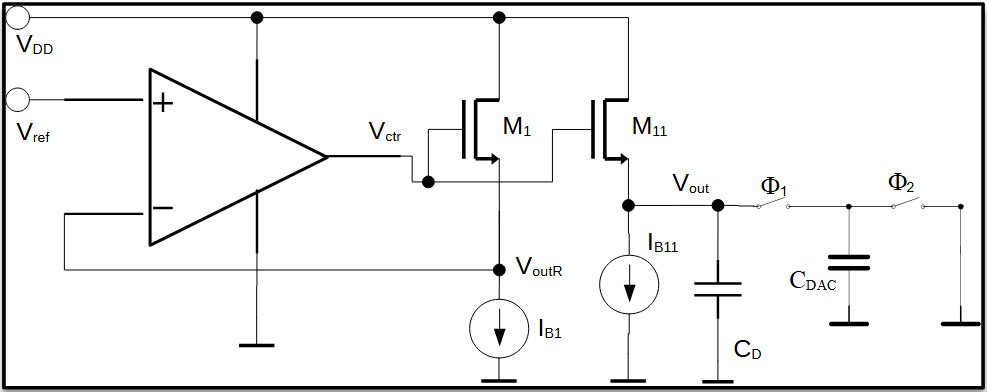
\includegraphics[width=0.8\linewidth]{IMAGENS/Reference buffer architecture.png}
    \caption{Arquitetura do buffer de referência.}
    \label{fig:arquitetura}
\end{figure}

A arquitetura adotada está representada na Fig.~\ref{fig:arquitetura}. O amplificador controla a
tensão $V_{ctr}$ de modo a que a saída do seguidor réplica $M_1$ ($V_{outR}$) seja igual a $V_{ref}$.
Como o seguidor de saída $M_{11}$ partilha a mesma tensão de gate e opera com a mesma densidade de corrente,
$V_{out}$ acompanha $V_{outR}$, sem que o transitório provocado pela ligação de $C_{DAC}$ perturbe diretamente a
malha de realimentação. O condensador $C_D$ funciona como reservatório de carga e limita a queda de tensão inicial.

\begin{figure}[H]
    \centering
    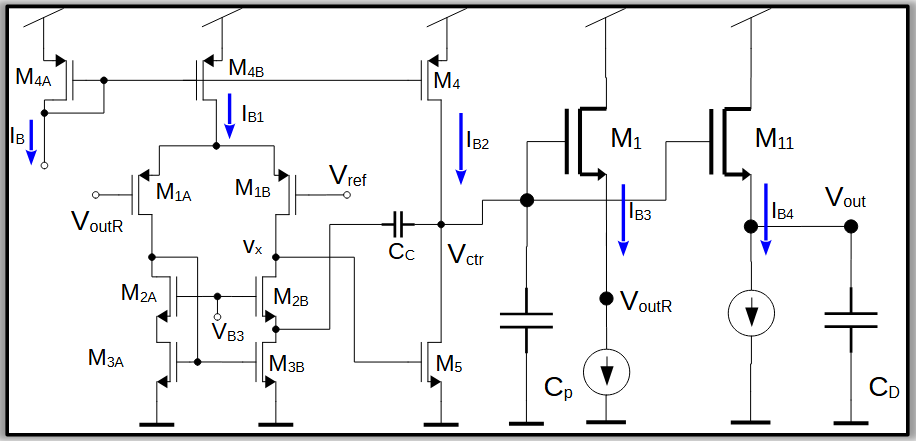
\includegraphics[width=0.9\linewidth]{IMAGENS/Suggested circuit.png}
    \caption{Circuito sugerido.}
    \label{fig:circuito}
\end{figure}

O circuito sugerido para o amplificador é apresentado na Fig.~\ref{fig:circuito}. A estabilidade é garantida por compensação indireta, com o condensador $C_C$ ligado entre
$V_{ctr}$ e a fonte do transístor de cascode $M_{2B}$.

O relatório está dividido em diversas partes. Na Secção~\ref{subsec:andar_saida} dimensiona-se o andar de saída
($M_{11}$, $C_D$ e a réplica $M_1$). Na Secção~\ref{subsec:analise_amp} analisa-se o amplificador e obtêm-se as
expressões do ganho, do GBW e dos polos. Na Secção~\ref{subsec:gmid} dimensionam-se os transístores pela metodologia
$g_m/I_D$. Nas secções seguintes apresentam-se os resultados de simulação: ponto de funcionamento, resposta em
frequência, impedância de saída, ruído, PSRR e funcionamento no tempo.